\setlength{\parskip}{1em}

\chapter{Úvodní obrazovka}

\section{Přihlášení}

Po otevření aplikace se zobrazí dialog pro přihlášení. První textové pole je pro přihlašovací jméno, které se automaticky převede na velká písmena, druhý je pro heslo. Tlačítkem \emph{OK} se uživatel přihlásí, tlačítkem \emph{Zrušit} se zruší přihlášení a dialog se zavře (viz obr. \ref{fig:login}). Přihlásit se může pouze uživatel s~pracovním poměrem na oddělení, ke kterému tablet patří. Pro práci s aplikací MediTab musí být uživatel vždy přihlášen!

\begin{figure}[H]
	\centering
	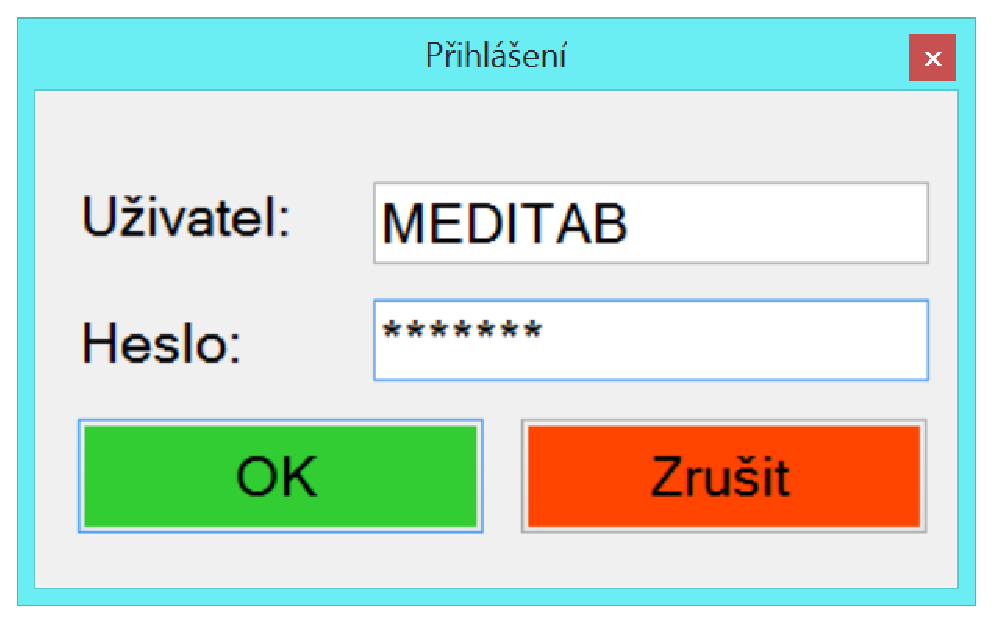
\includegraphics[width=0.5\textwidth]{img/login.eps}
	\caption{Přihlášení}
  \label{fig:login}
\end{figure}

Přihlášený uživatel se může odhlásit kliknutím na tlačítko \emph{Odhlásit}, které se nachází na horní liště úvodní obrazovky.

\section{Výběr pacienta}

Po přihlášení uživatele se načte seznam pacientů hospitalizovaných na oddělení (viz obr. \ref{fig:main}). Výběrem řádky s pacientem se otevře karta pacienta.
Tlačítko \emph{Konec} odhlásí aktuálního uživatele a aplikaci ukončí. Tlačítko \emph{Odhlásit} odhlásí aktuálně přihlášeného uživatele a otevře dialog pro přihlášení nového uživatele.

\begin{figure}[H]
	\centering
	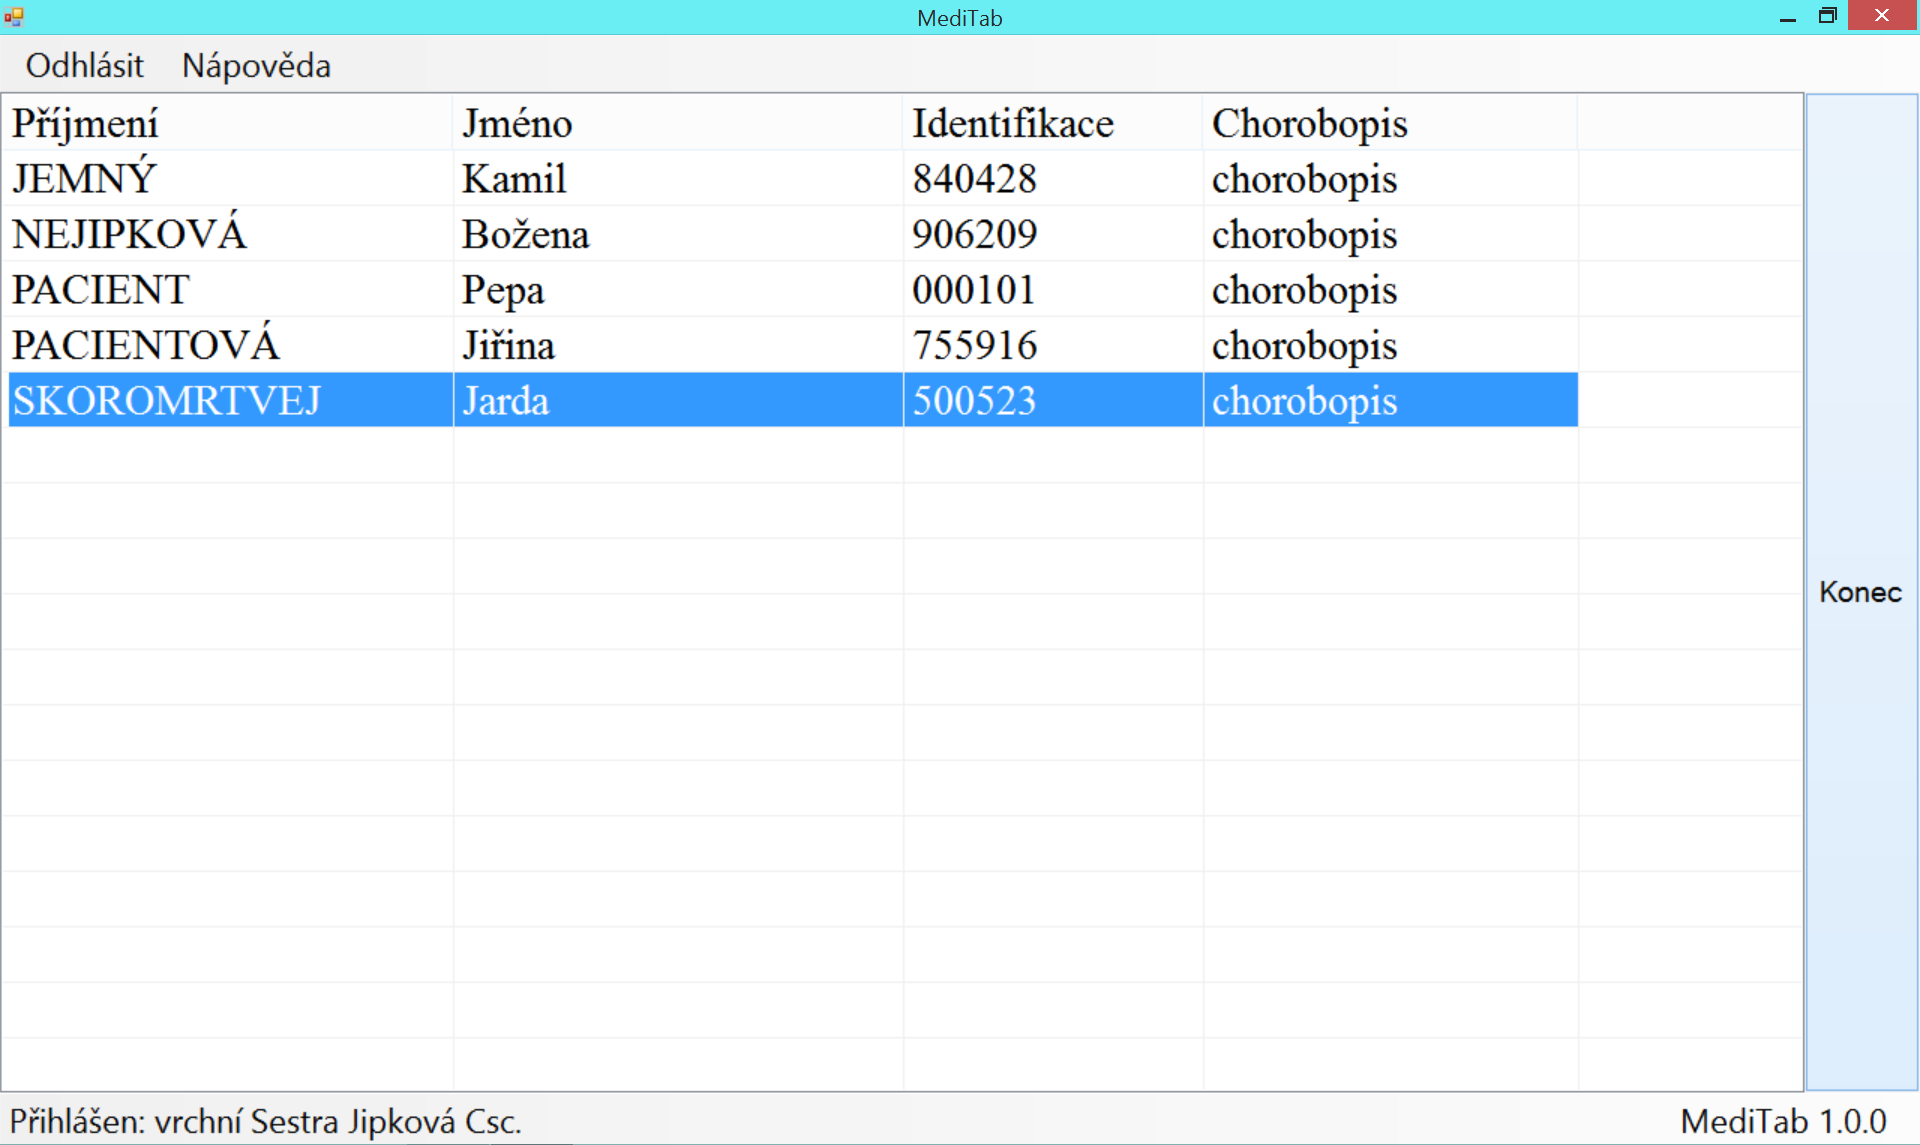
\includegraphics[width=1\textwidth]{img/main.eps}
	\caption{Úvodní obrazovka}
  \label{fig:main}
\end{figure}

%%%%%%%%%%%%%%%%%%%%%%%%%%%%%%%%%%%%%%%%%%%%%%%%%%%%%%%%%%%%%%%%%%%%%%%%%%%%%%%%%%%%%%%%%%%%%%%%%%%%

\chapter{Karta pacienta}

Karta pacienta má 5 záložek: \emph{Medikační karta}, \emph{Denní bilance tekutin}, \emph{Hodinová bilance tekutin}, \emph{Invazivní přístupy}, \emph{Fyziologie}. Tlačítkem \emph{Zpět} se vrátí k výběru pacienta. Tlačítko \emph{Opravy} otevře okno oprav, kde je možné vrátit provedené akce (viz kapitola \ref{ch:opravy}). V dolní liště je jméno přihlášeného uživatele a jméno vybraného pacienta.

%%%%%%%%%%%%%%%%%%%%%%%%%%%%%%%%%%%%%%%%%%%%%%%%%%%%%%%%%%%%%%%%%%%%%%%%%%%%%%%%%%%%%%%%%%%%%%%%%%%%

\section{Medikační karta}

Záložka medikační karty nahrazuje tištěnou formu medikační karty. Jedná se o tabulku s názvy léku, předepsaným dávkováním a jednotlivými hodinami dávkování (viz obr. \ref{fig:medikace}). V prvním sloupci je název léku, v druhém předepsané dávkování. Červeně označený lék znamená, že se jedná o opiát, modře označené dávkování značí, že u dávkování je připsaná poznámka. Další sloupce značí jednotlivé hodiny s předepsanými ordinacemi. Sloupec aktuální hodiny je zvýrazněn khaki barvou. 

Barvy polí:
\parskip=0em
\begin{itemize}
	\item Zeleně - provedená ordinace.
	\item Světle zeleně - provedená infuze (kromě hodiny, kdy infuze začíná, to je tmavě zelené). Infuze může mít definovaný konec, nebo je zobrazena do aktuální hodiny.
	\item Šedě - předepsaná ordinace.
	\item Fialově - neprovedená ordinace.
\end{itemize}
\parskip=1em

\begin{figure}[H]
	\centering
	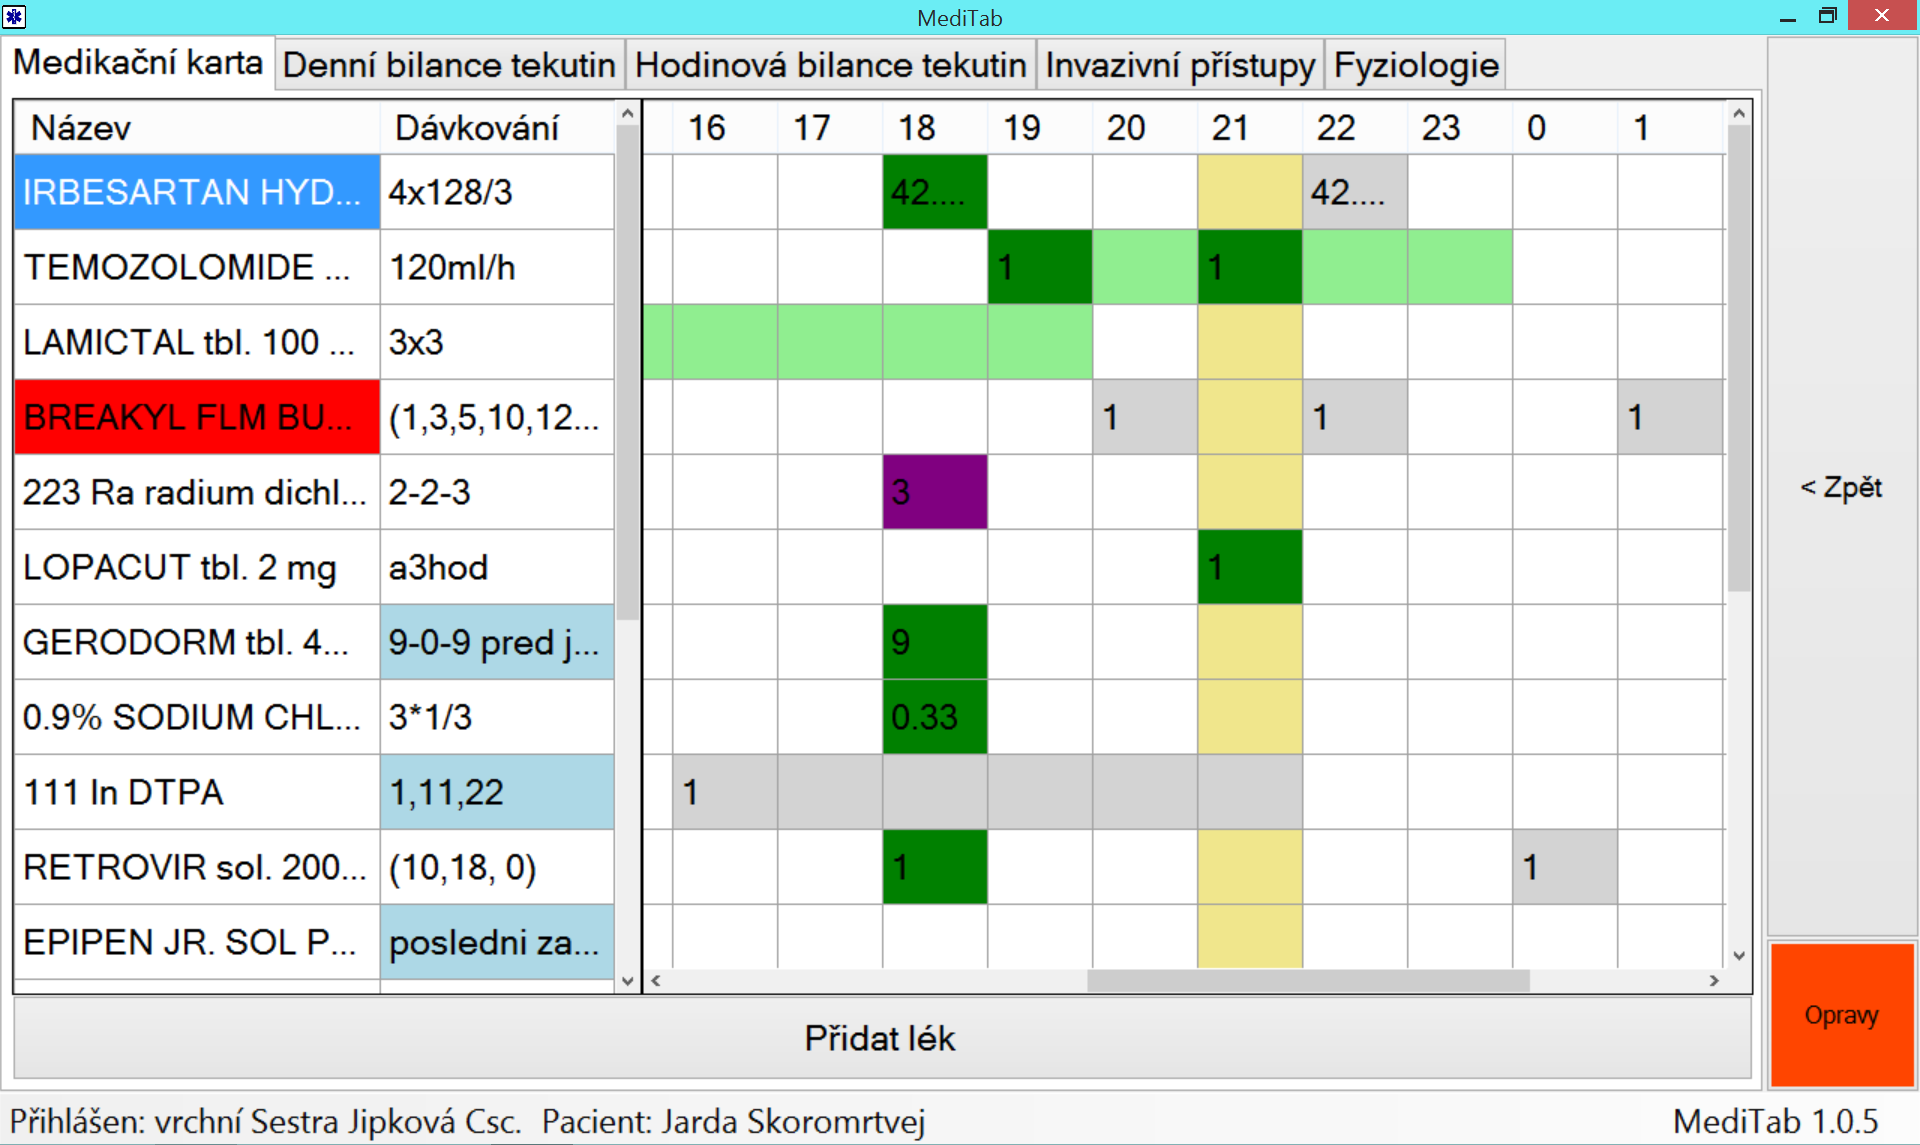
\includegraphics[width=1\textwidth]{img/medikace.eps}
	\caption{Medikační karta}
  \label{fig:medikace}
\end{figure}

Kliknutím na ordinaci se zobrazí dialog pro zadání podání ordinací (viz kapitola \ref{sec:ordinace}). Dvojitým kliknutím se provede podání jednorázové ordinace (neplatí u infuzí).

Tabulka se posouvá dvěma prsty. Spodní tlačítko je pro přidání nového léku (viz kapitola \ref{sec:pridat_lek}).

\subsection{Podání ordinací}
\label{sec:ordinace}

Dialog podání ordinací (obr. \ref{fig:ordinace}) zobrazuje seznam ordinací daného léku (vlevo). Vybráním ordinace ze seznamu se zobrazí její detail (vpravo). Ordinace se dá upravovat. Kliknutím na tlačítko \emph{Podat} se provede okamžité podání ordinace, na tlačítko \emph{Nepodat} nepodání ordinace. Hodiny podání se mění přejetím prstu po poli s časem. Pro zadání času konce infuze musí být zaškrtnuto pole \emph{konec}. Stav podání a~jednotky se vybírají ze seznamu. Do poznámky lze zapisovat pouze, pokud lék nebyl podán.

Kliknutím na tlačítko \emph{Přidat} se k léku přidá nová ordinace, kliknutím na tlačítko \emph{Smazat} se smaže právě vybraná ordinace.

\begin{figure}[H]
	\centering
	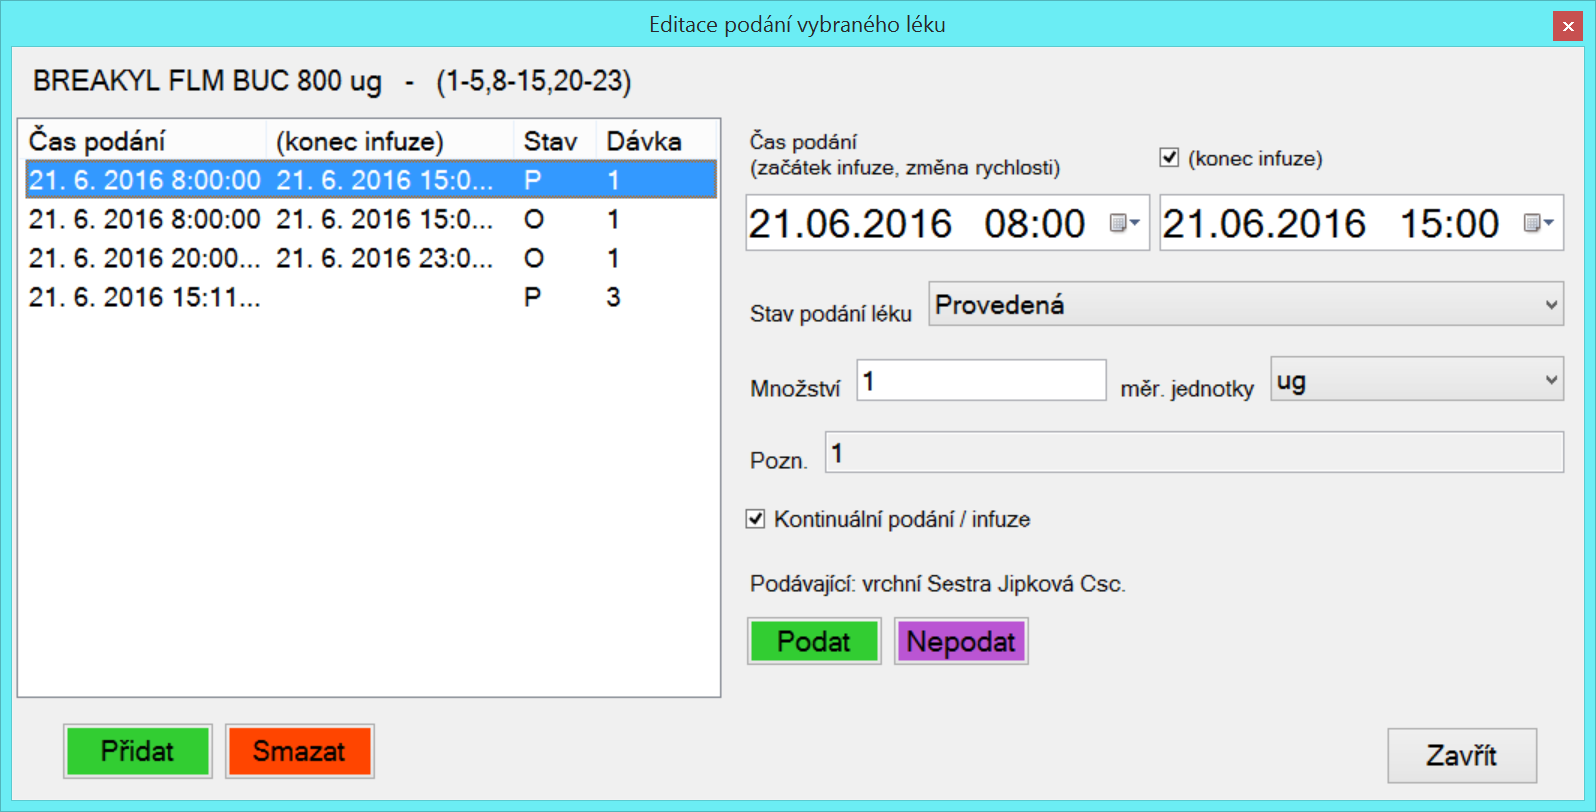
\includegraphics[width=0.8\textwidth]{img/ordinace.eps}
	\caption{Dialog podání ordinací}
  \label{fig:ordinace}
\end{figure}


\subsection{Přidání léku}
\label{sec:pridat_lek}

Aplikace nabízí možnost přidání nového léku, který byl lékařem předepsán a není v klinické události. Kliknutím na tlačítko \emph{Přidat lék} se zobrazí dialog přidání nového léku (viz obr. \ref{fig:pridat_lek}).

\begin{figure}[H]
	\centering
	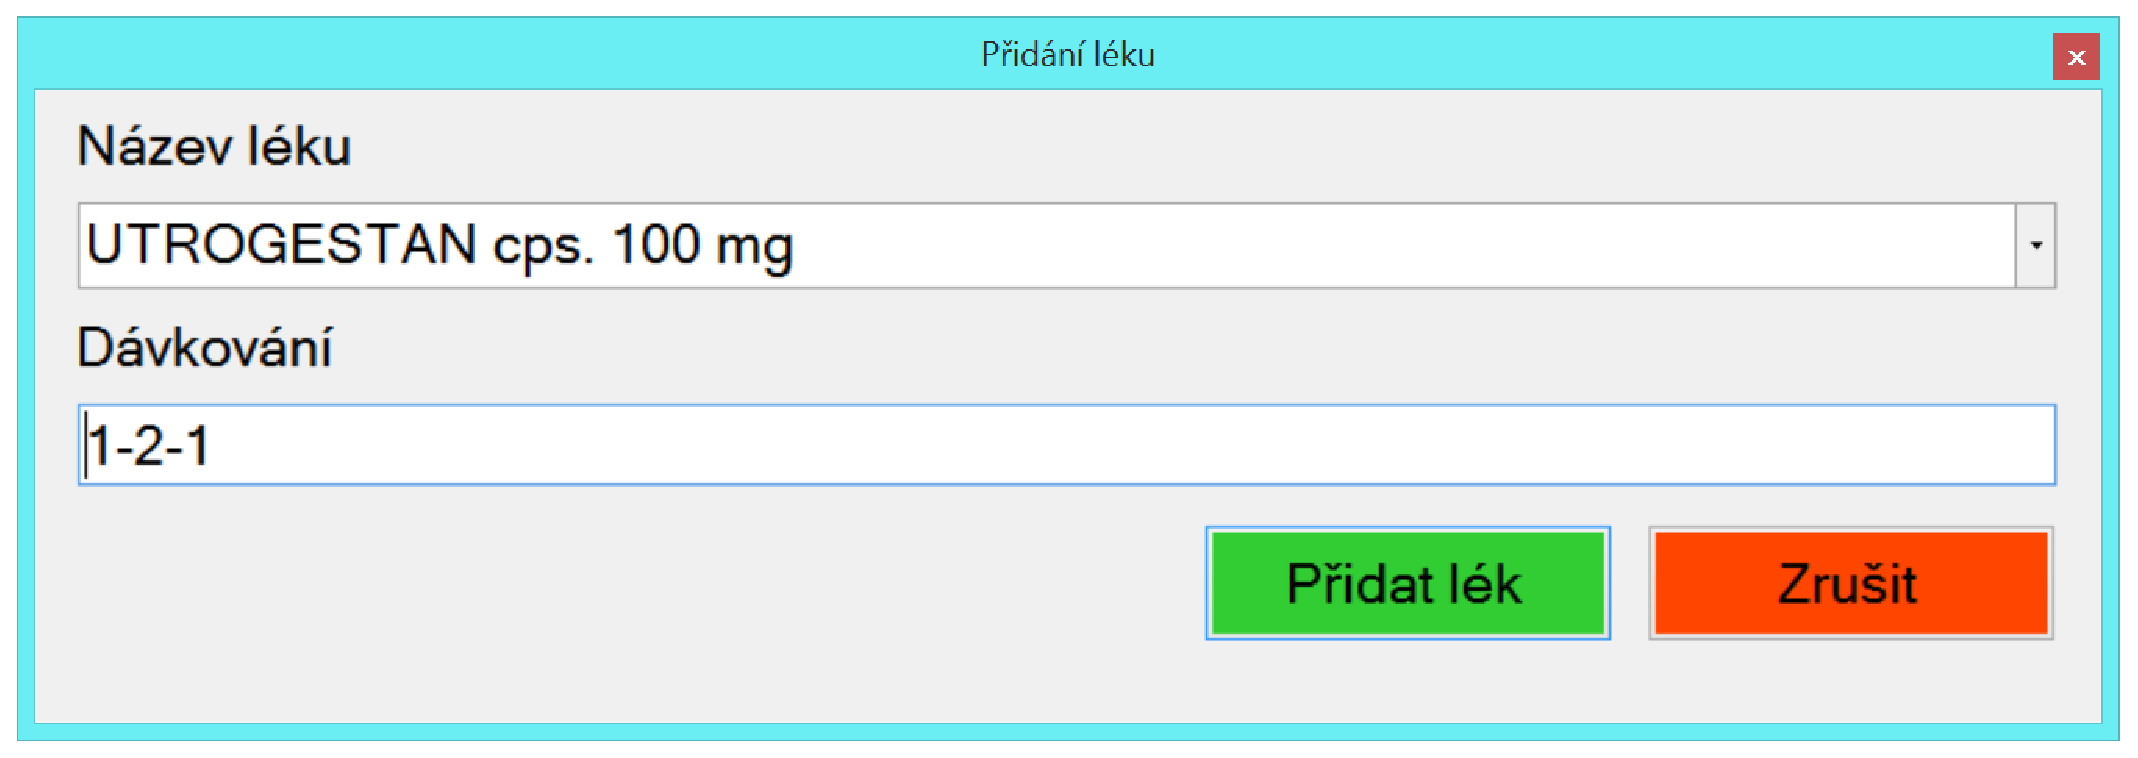
\includegraphics[width=0.8\textwidth]{img/medikace_pridat_lek.eps}
	\caption{Dialog přidání léku}
  \label{fig:pridat_lek}
\end{figure}

Do prvního pole se zadává lék. Kliknutím na pole se zobrazí klávesnice. Stačí napsat pouze část názvu léku. Po zavření klávesnice se vyhledají všechny léky obsahující část názvu a zobrazí se jejich seznam. Kliknutím na položku seznamu se vybere požadovaný lék.

Druhé pole je k zadání dávkování. Dávkování by mělo být zapsané dle standartů nemocnice.

%%%%%%%%%%%%%%%%%%%%%%%%%%%%%%%%%%%%%%%%%%%%%%%%%%%%%%%%%%%%%%%%%%%%%%%%%%%%%%%%%%%%%%%%%%%%%%%%%%%%

\section{Bilance tekutin}

V záložkách bilance tekutin se zaznamenávají veškeré příjmy a výdaje tekutin. Záložky jsou rozděleny na dvě části. Vlevo zeleně jsou tekutiny příjmu, vpravo červeně tekutiny výdeje. U každé tekutiny jsou pole pro zadávání hodnot. Po kliknutí na pole se zobrazí numerická klávesnice.


\subsection{Denní bilance tekutin}

U každé tekutiny jsou dvě pole. První zobrazuje celkový součet za den, druhý je pro zadání nové hodnoty. Novou hodnotu lze zadat přepsáním hodnoty v prvním poli (nová hodnota musí být větší než původní), nebo zadáním naměřené hodnoty do druhého pole, hodnota se přičte k původní (v prvním sloupci). Zaznamenané hodnoty se musí potvrdit kliknutím na tlačítko \emph{Uložit}.

\begin{figure}[H]
	\centering
	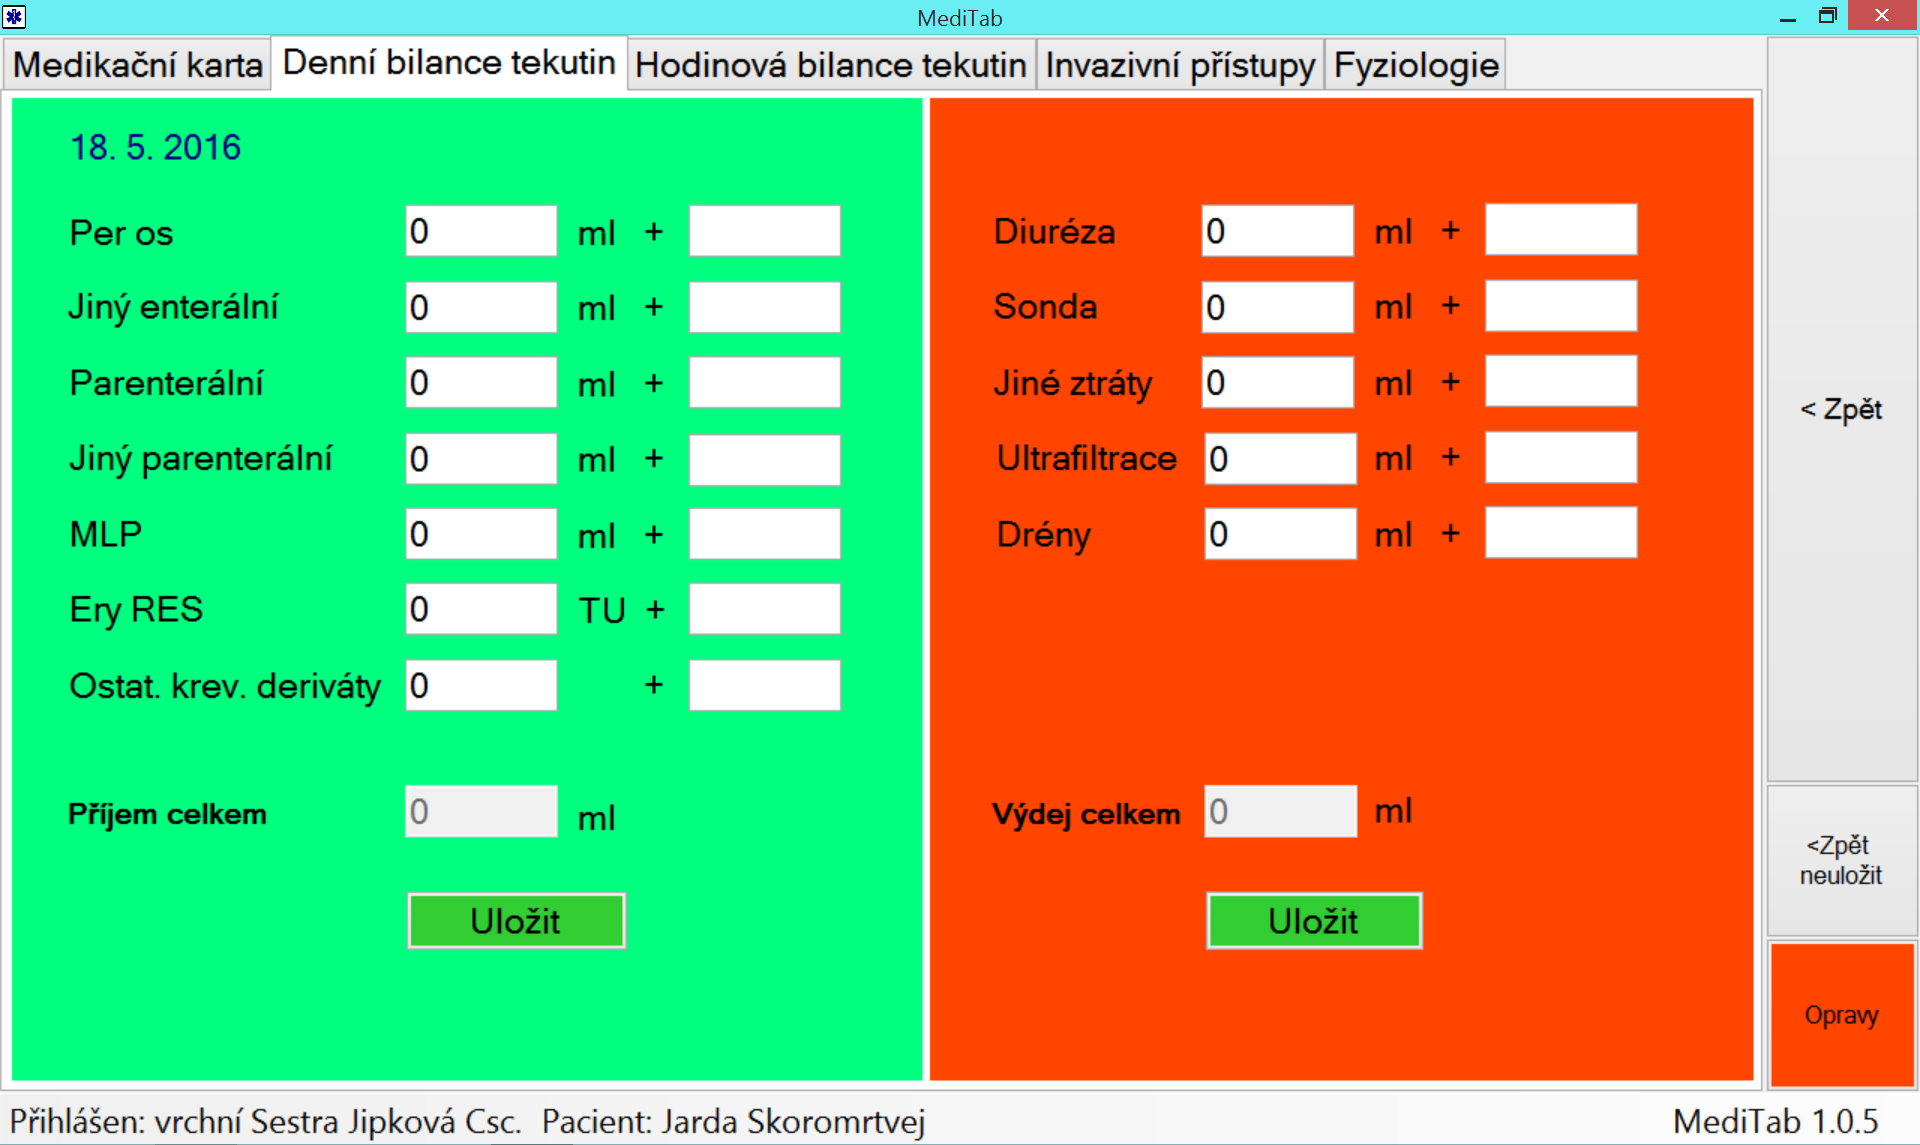
\includegraphics[width=1\textwidth]{img/bilance_den.eps}
	\caption{Denní bilance tekutin}
  \label{fig:bilance}
\end{figure}

\subsection{Hodinová bilance tekutin}

U každé tekutiny je pole pro zadání hodnoty v aktuální hodinu a tlačítko k zobrazení tabulky všech hodin. Po zobrazení tabulky lze zadávat hodnoty i zpětně, aktuální hodina je v tabulce vyznačena khaki barvou. Hodnotu lze zadat pouze jedenkrát v každé hodině. Zaznamenané hodnoty se musí potvrdit kliknutím na tlačítko \emph{Uložit}.

\begin{figure}[H]
	\centering
	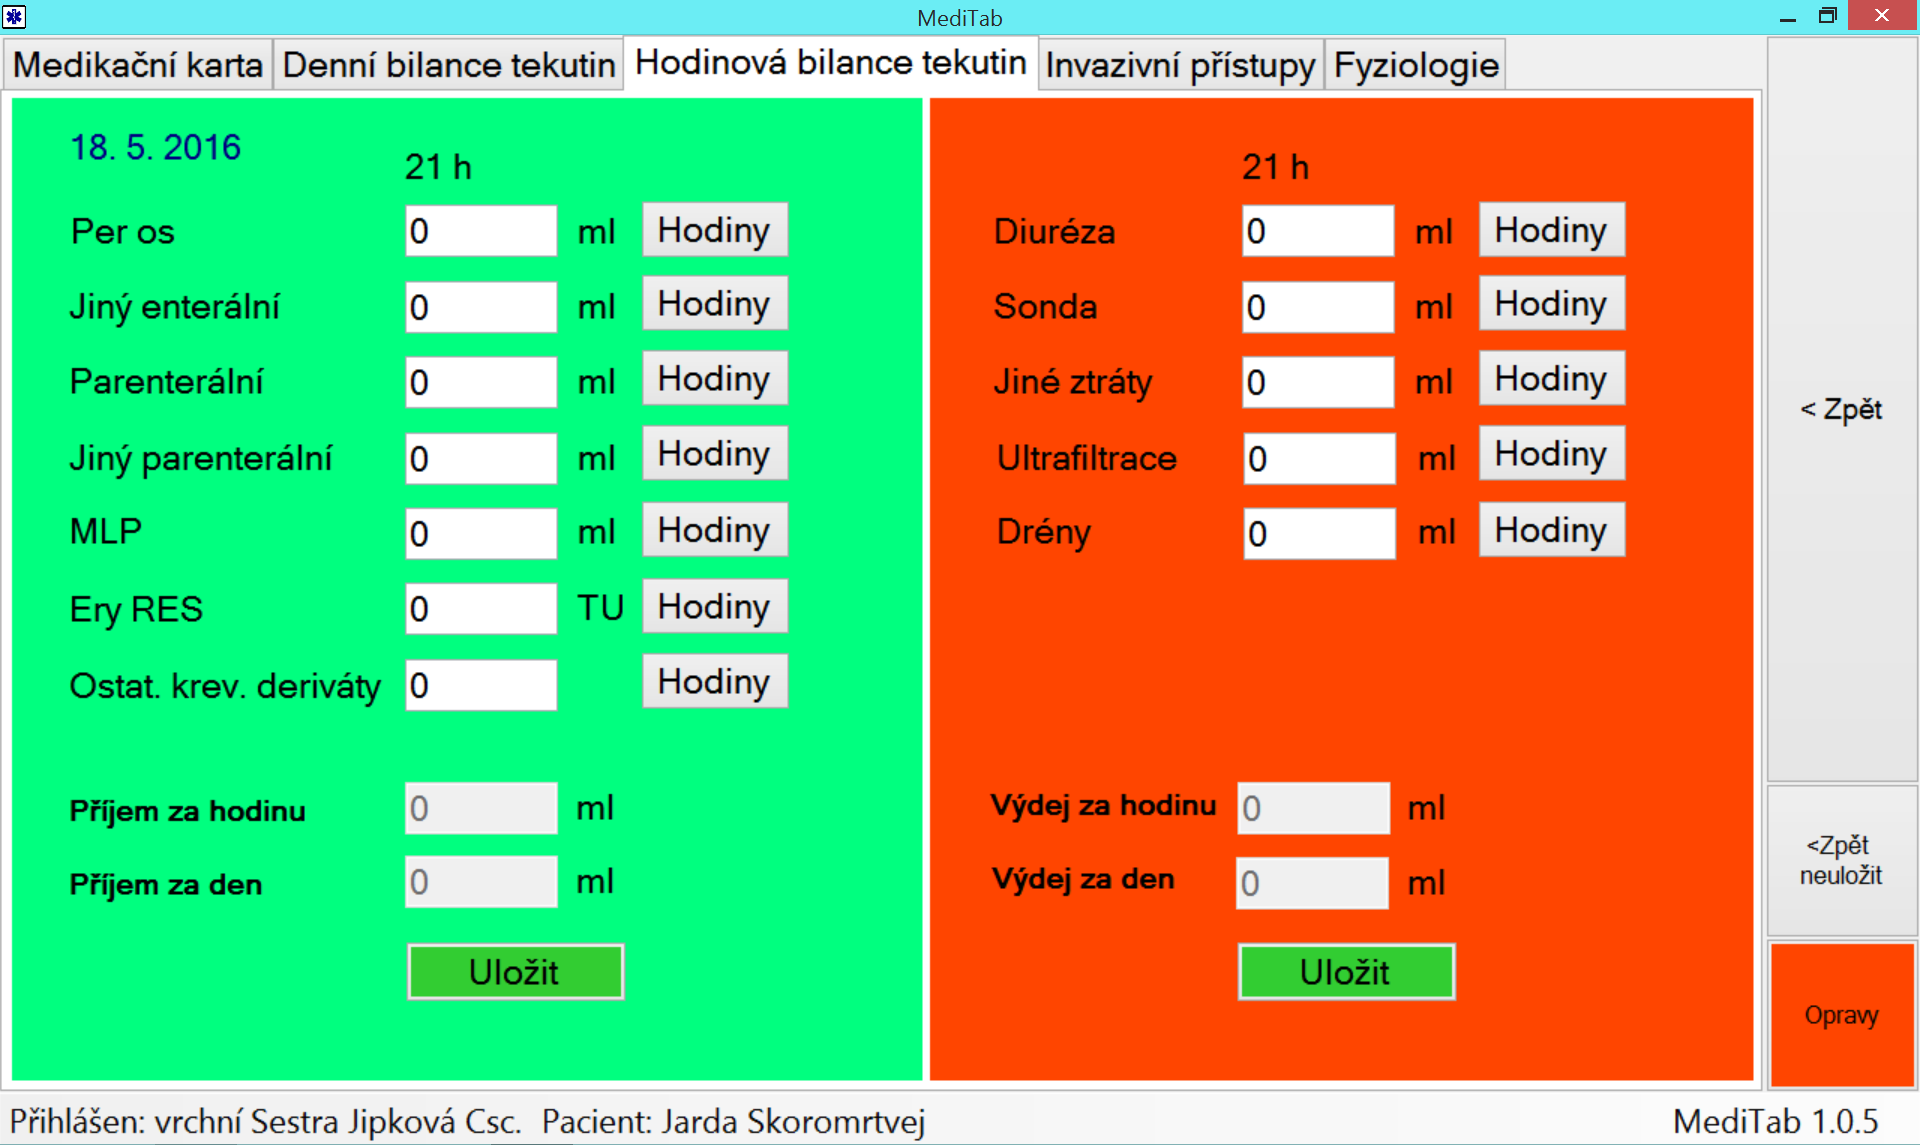
\includegraphics[width=1\textwidth]{img/bilance_hod.eps}
	\caption{Hodinová bilance tekutin}
  \label{fig:bilance_hod}
\end{figure}

%%%%%%%%%%%%%%%%%%%%%%%%%%%%%%%%%%%%%%%%%%%%%%%%%%%%%%%%%%%%%%%%%%%%%%%%%%%%%%%%%%%%%%%%%%%%%%%%%%%%

\section{Invazivní přístupy}

V záložce je seznam invazivních přístupů zavedených pacientovi (viz obr. \ref{fig:pristupy}). Červeně označená položka značí požadavek na výměnu invazivního přístupu. Poslední položkou v seznamu invazivních přístupů je možnost přidání nového přístupu (viz kapitola \ref{sec:pridat_pristup}). Seznam se posouvá tažením jedním prstem vedle položek seznamu.

Tlačítka:
\parskip=0em
\begin{itemize}
	\item \emph{Vyměnit}		-	zadá/zruší požadavek na výměnu invazivního přístupu (položka zčervená)
	\item \emph{Aktualizuj}	-	provede výměnu invazivního přístupu (datum se nastaví na aktualní den a počet dnů na 1)
	\item \emph{Vymaž}			-	smaže invazivní přístup
\end{itemize}

\begin{figure}[H]
	\centering
	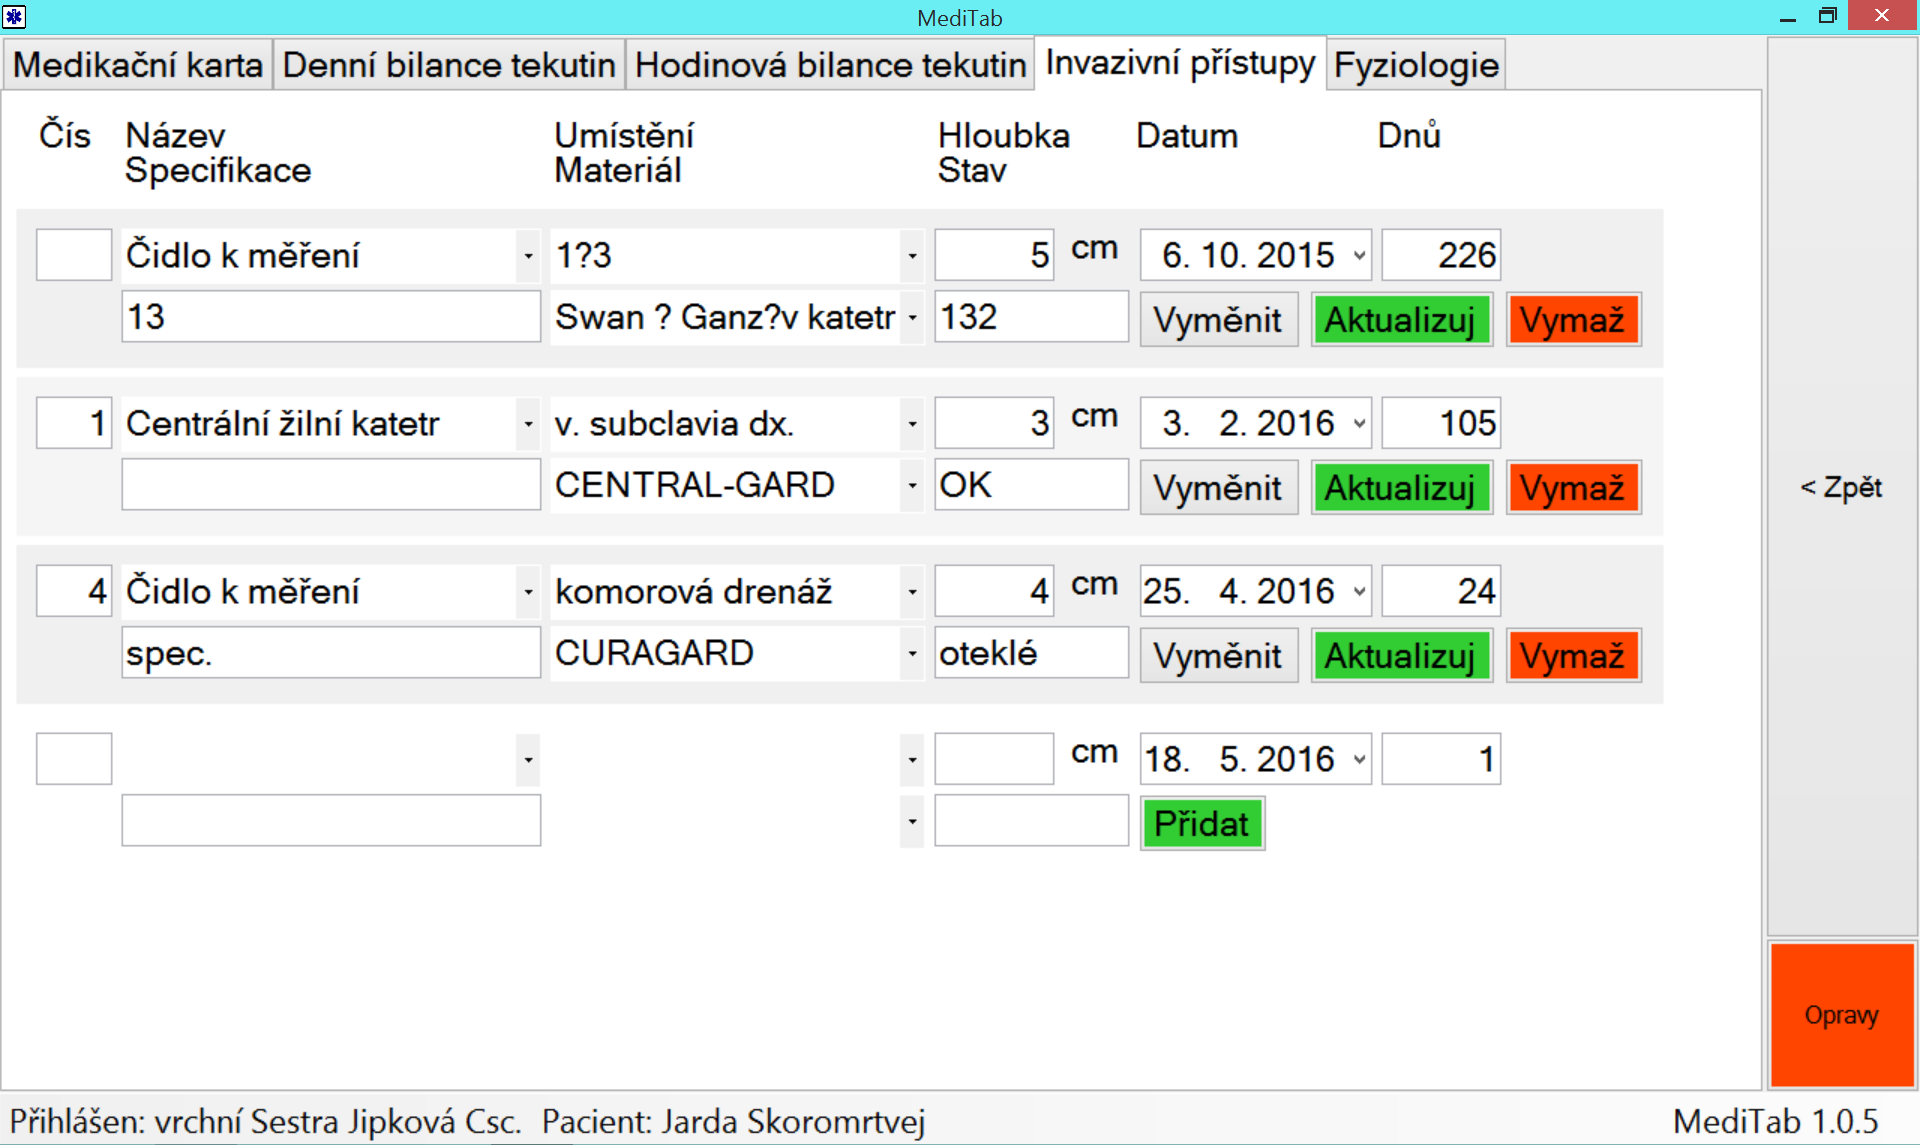
\includegraphics[width=1\textwidth]{img/invaz_pristup.eps}
	\caption{Invazivní přístupy}
  \label{fig:pristupy}
\end{figure}
\parskip=1em

\subsection{Přidání nového invazivního přístupu}
\label{sec:pridat_pristup}

Poslední položkou v seznamu invazivních přístupů je možnost přidání nového invazivního přístupu. Název invazivního přístupu a materiál se vybírá ze seznamu. Umístění se vybírá ze seznamu dle typu invazivního přístupu, nebo lze zadat jiné umístění. Datum je automaticky nastaven na aktuální den a počet dnů na 1. Číslo invazivního přístupu a hloubka zavedení jsou číselné hodnoty. Zbytek polí jsou textové hodnoty pro specifikování invazivního přístupu.

Přidání invazivního přístupu se provede kliknutím na tlačítko \emph{Přidat}.

%%%%%%%%%%%%%%%%%%%%%%%%%%%%%%%%%%%%%%%%%%%%%%%%%%%%%%%%%%%%%%%%%%%%%%%%%%%%%%%%%%%%%%%%%%%%%%%%%%%%

\section{Fyziologie}

V záložce je seznam záznamů o životních funkcích pacienta.

\begin{itemize}
	\item Datum záznamu
	\item Teplota
	\item STK
	\item DTK
	\item Tep
	\item Dech
\end{itemize}

Záznam lze upravit přepsáním hodnot a kliknutím na tlačítko \emph{Upravit}, nebo smazat tlačítkem \emph{Smazat}.

\begin{figure}[H]
	\centering
	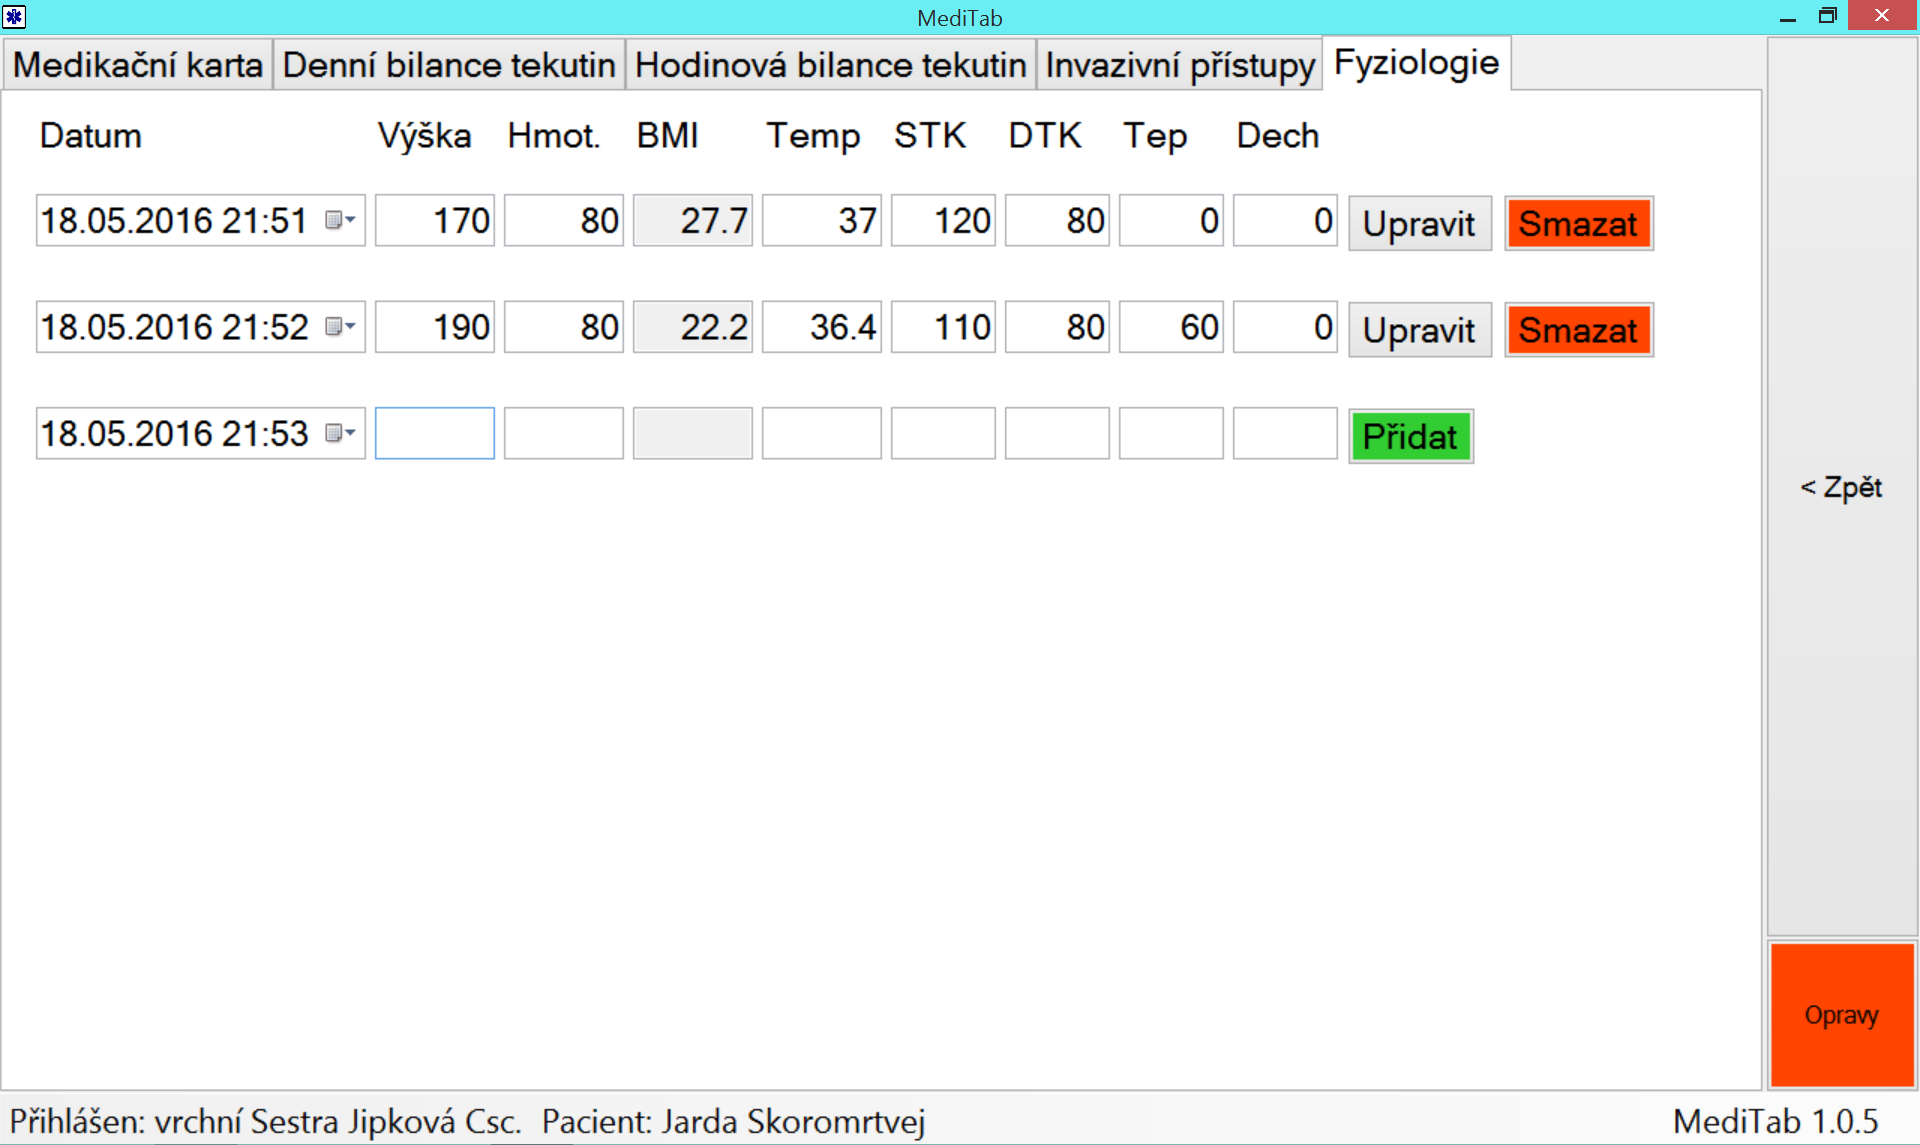
\includegraphics[width=1\textwidth]{img/fyziologie.eps}
	\caption{Fyziologie}
  \label{fig:fyziologie}
\end{figure}

Poslední položkou je možnost přidání nového záznamu. Po zapsání naměřených hodnot se záznam uloží kliknutím na tlačítko \emph{Přidat}.

Seznam se posouvá tažením jedním prstem vedle položek seznamu.

%%%%%%%%%%%%%%%%%%%%%%%%%%%%%%%%%%%%%%%%%%%%%%%%%%%%%%%%%%%%%%%%%%%%%%%%%%%%%%%%%%%%%%%%%%%%%%%%%%%%

\chapter{Opravy}
\label{ch:opravy}

Kliknutím na tlačítko \emph{Opravy} na kartě pacienta se zobrazí okno se seznamem možných oprav právě otevřené záložky (viz obr. \ref{fig:opravy}). Zrušení provedené operace se provede kliknutím na křížek u každé položky.

\begin{figure}[H]
	\centering
	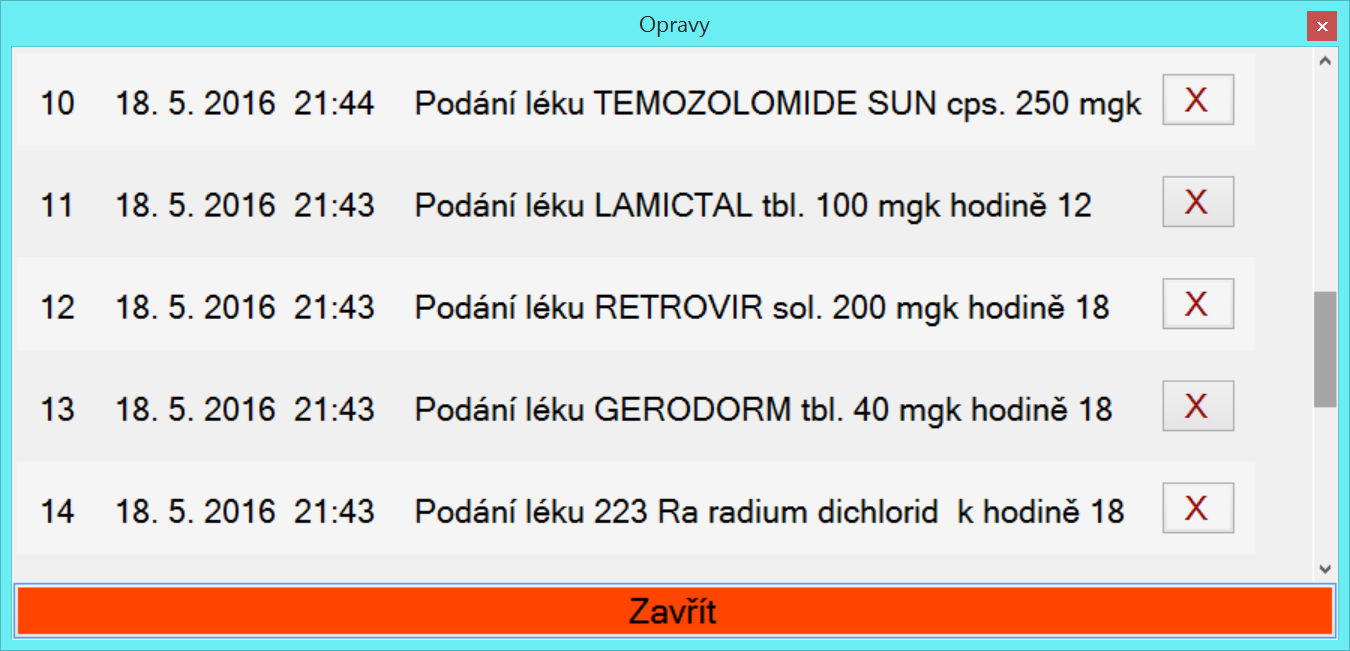
\includegraphics[width=0.7\textwidth]{img/opravy.eps}
	\caption{Dialog oprav}
  \label{fig:opravy}
\end{figure}
